\newpage
\section{Demonstrating Example}
\label{sec:demonstratingexample}

To illustrate the \Compose* toolset, this section introduces a \emph{Pac-Man} example.
The Pac-Man game is a classic arcade game in which the user, represented by Pac-Man, moves in a maze to eat pills.
Meanwhile, a number of ghosts try to catch and eat Pac-Man.
There are, however, four power pills in the maze that make Pac-Man evil. In its evil state, Pac-Man can eat ghosts.

A simple list of requirements for the Pac-Man game is briefly discussed here:
\begin{itemize}[noitemsep]
  \item The number of lives taken from Pac-Man when eaten by a ghost;
  \item A game should end when Pac-Man has no more lives;
  \item The score of a game should increase when Pac-Man eats a pill or a ghost;
  \item A user should be able to use a keyboard to move Pac-Man around the maze;
  \item Ghosts should know whether Pac-Man is evil or not;
  \item Ghosts should know where Pac-Man is located;
  \item Ghosts should, depending on the state of Pac-Man, hunt or flee from Pac-Man;
  \item At fixed intervals a bonus item should appear that gives bonus points when eaten by Pac-Man.
\end{itemize}

\subsection{Initial Object-Oriented Design}

\begin{figure}[p]
  \centering
  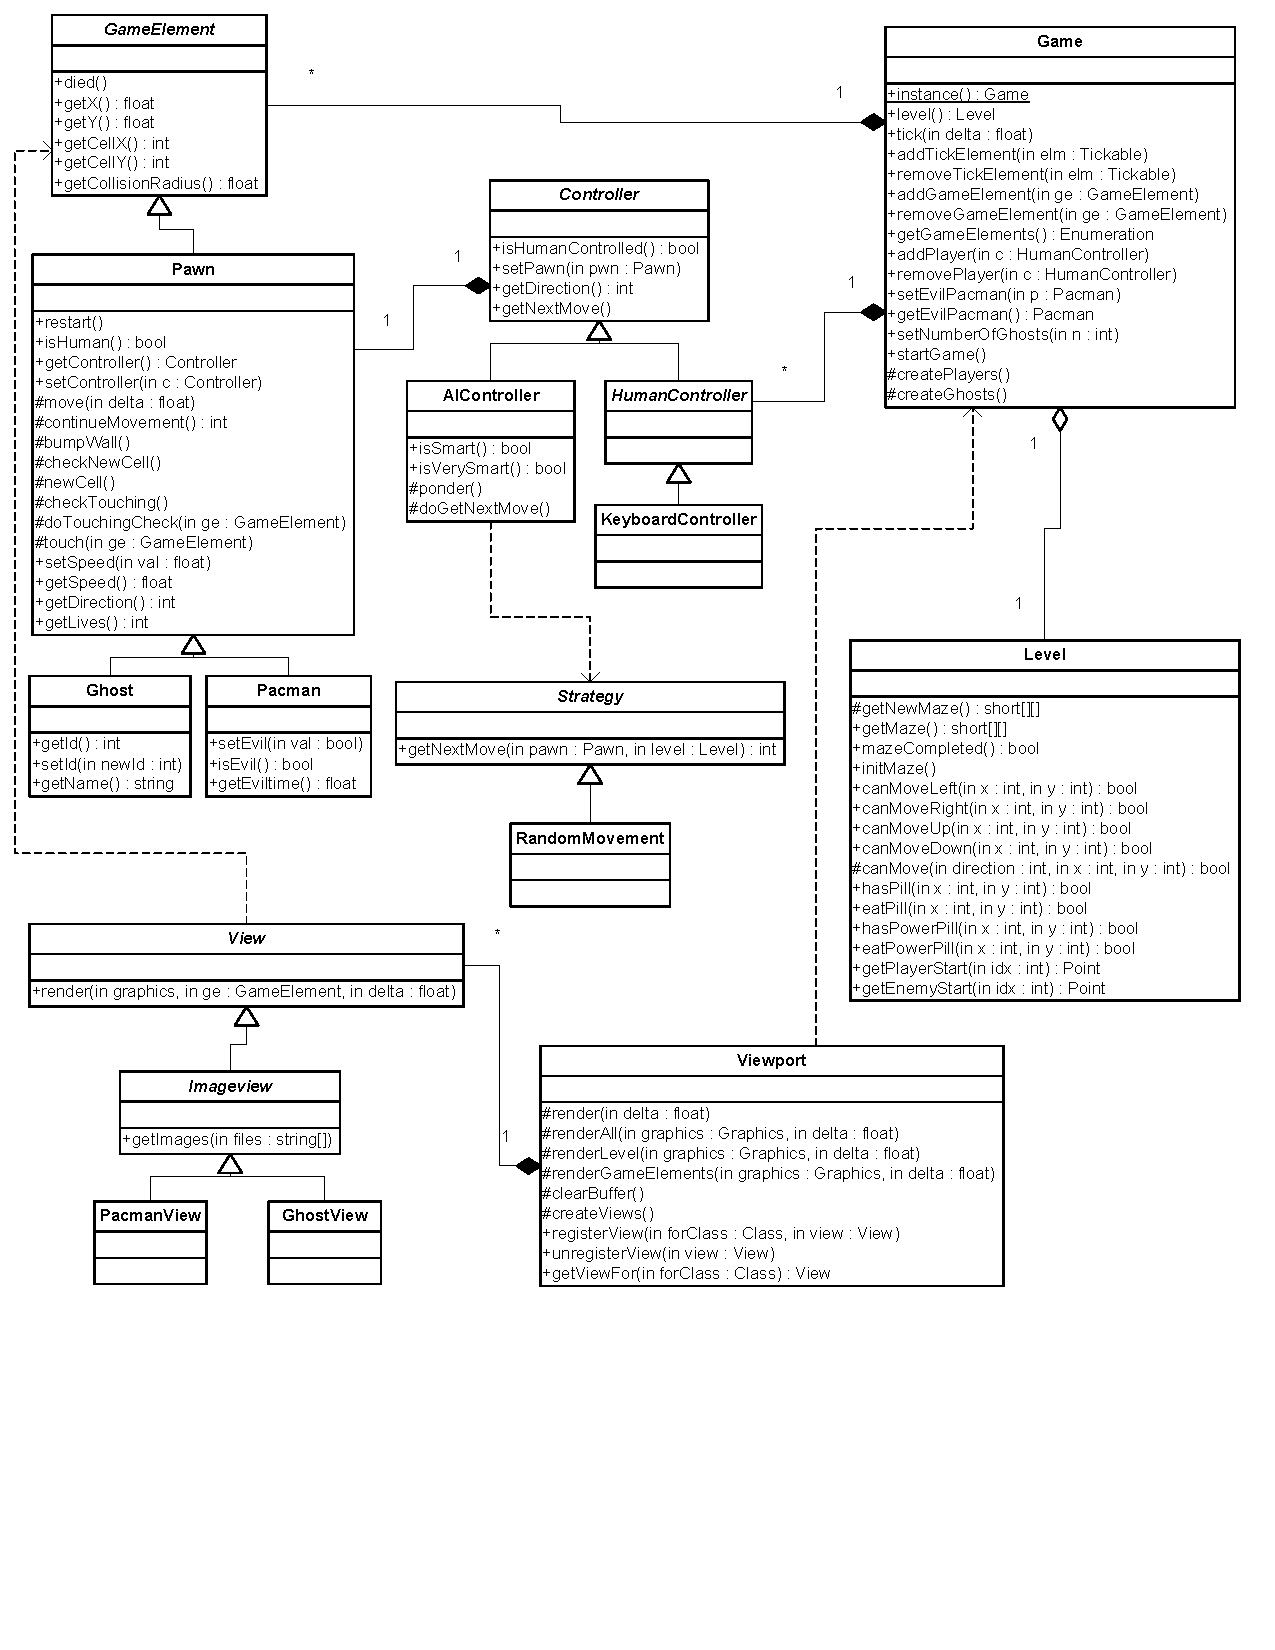
\includegraphics[style=page]{PacmanTwo}
  \caption{Class diagram of the object-oriented Pac-Man game}
  \label{fig:pacman2_class_diagram}
\end{figure}

\nomenclature{UML}{Unified Modeling Language}%
\autoref{fig:pacman2_class_diagram} shows an initial object-oriented design for the Pac-Man game.
Note that this UML class diagram does not show the class attributes.
The classes in this diagram are:
\begin{description}[noitemsep,style=sameline,leftmargin=32mm]
	\item[AIController] The \lstinline|AIController| is used for the non human controlled pawns. It makes
		use of the \lstinline|Strategy| class	to determine the next move;
	\item[Controller] The controller is responsible for providing the \lstinline|Pawn| the desired direction of movement;
	\item[Game] This class encapsulates the control flow and controls the state of a game;
	\item[GameElement] This is the base class for all visual elements in the game, with the exception of the pills;
		A \lstinline|GameElement| has a position within the level and a collision radius;
	\item[Ghost] This class is a representation of a ghost chasing Pac-Man. Each ghost has an identifier that can be
		to change the behavior for individual ghosts;		
	\item[HumanController] The \lstinline|HumanController| is a controller class that receives movement instructions
		from the player;
	\item[KeyboardController] The \lstinline|KeyboardController| is an implementation that reads the instructions 
		from the keyboard;			
	\item[Level] This class contains the structural information of the maze including information about the pills;		
	\item[Pacman] This is a representation of the user controlled pawn in the game. It contains a flag that tells if
		the Pac-Man is in evil mode;	
	\item[Pawn] The \lstinline|Pawn| class is used for all non stationary \lstinline|GameElement|. Pawns are 
		controlled by an instance of the \lstinline|Controller| class and has a speed, direction and number of lives.
		The pawn performs collision checks on every move and acts accordingly;
	\item[RandomMovement] The \lstinline|RandomMovement| class is returns a random direction the given 
		pawn can move to;
	\item[Strategy] This class is used by the \lstinline|AIController| to make a movement choice;
	\item[View] \lstinline|GameElements| are drawn on the \lstinline|Viewport| using a View 
		implementation. Each \lstinline|GameElement| implementation has	its own View subclass;
	\item[Viewport] The \lstinline|Viewport| shows the current game to the player. It is responsible for rendering 
		the maze. 
\end{description}

\subsection{Completing the Pac-Man Example}

The initial object-oriented design, described in the previous section, does not implement all the stated system requirements.
The missing requirements are:
\begin{itemize}[noitemsep]
  \samepage
  \item The application does not maintain a score for the user;
  \item Ghosts move in random directions instead of chasing or fleeing from Pac-Man;
  \item There is no bonus item that Pac-Man can pick up.
\end{itemize}
In the next sections, we describe why and how to implement these requirements in the \Compose* language.

\subsubsection{Implementation of Scoring}

The first system requirement that we need to add to the existing Pac-Man game is scoring.
This concern involves a number of events.
The score should be updated whenever Pac-Man eats a pill, power pill or ghost.
And the score itself has to be drawn on the screen to relay it back to the user.
These events scatter over multiple classes: \lstinline|Level| (updating score), \lstinline|Ghost| (updating score), \lstinline|Viewport| (drawning score).
Thus scoring is an example of a crosscutting concern. 

To implement scoring in the \Compose* language, we divide the implementation into two parts.
The first part is a \Compose* concern definition stating which filter modules to superimpose.
\autoref{lst:scoringconcern} shows an example \Compose* concern definition of scoring.

\begin{lstlisting}[style=floatlisting,escapeinside={&$}{$&},language=ComposeStar,%
                   caption={\expandafter{\lstinline[style=inline]|Scoring|} concern in \Compose*{}},%
                   label={lst:scoringconcern}]
concern Scoring in PacmanTwo&$\label{line:scoring_concern}$&
{
	filtermodule registerScorePawns&$\label{line:scoring_fm_rsp}$&
	{
		externals
			score : PacmanTwo.Scoring.Score = PacmanTwo.Scoring.Score.instance();
		inputfilters
			scored : After = { [*.died] score.pawnDied }&$\label{line:scoring_fm_rsp_scored}$&
	}&$\label{line:scoring_fm_rsp_end}$&

	filtermodule registerScoreLevel&$\label{line:scoring_fm_rsl}$&
	{
		externals
			score : PacmanTwo.Scoring.Score = PacmanTwo.Scoring.Score.instance();
		inputfilters
			scored : After = { [*.eatPill] score.eatPill
			                 , [*.eatPowerPill] score.eatPowerPill }
	}&$\label{line:scoring_fm_rsl_end}$&

	filtermodule renderScore&$\label{line:scoring_fm_rs}$&
	{
		internals
			scoreview : PacmanTwo.Scoring.ScoreView;
		inputfilters
			render : After = { [*.renderAll] scoreview.renderScore }
	}&$\label{line:scoring_fm_rs_end}$&

	superimposition&$\label{line:scoring_si}$&
	{
		selectors
			lvl = { C | isClassWithName(C, 'PacmanTwo.Level') };
			pawns = { C | isClassWithNameInList(C, ['PacmanTwo.Ghost']) };
			viewport = { C | isClassWithName(C, 'PacmanTwo.GUI.Viewport' ) };
		filtermodules
			lvl <- registerScoreLevel;
			pawns <- registerScorePawns;
			viewport <- renderScore;
	}&$\label{line:scoring_si_end}$&
}
\end{lstlisting}

This concern definition is called \lstinline|Scoring| (line~\ref{line:scoring_concern}) and contains two parts.
The first part is the declaration of the filter modules called \lstinline|registerScorePawns| (lines~\ref{line:scoring_fm_rsp}--\ref{line:scoring_fm_rsp_end}), \lstinline|registerScoreLevel| (lines~\ref{line:scoring_fm_rsl}--\ref{line:scoring_fm_rsl_end}), and \lstinline|renderScore| (lines~\ref{line:scoring_fm_rs}--\ref{line:scoring_fm_rs_end}).
The first two filter modules \lstinline|registerScorePawns| and \lstinline|registerScoreLevel| will update the current score. When Pac-Man eats a ghost the \lstinline|died| method will be called on the \lstinline|Ghost|. The filter module \lstinline|registerScorePawns| contains an \emph{after filter} called \lstinline|scored| (line~\ref{line:scoring_fm_rsp_scored}). This filter will send a message to the \lstinline|Score| instance when the \lstinline|died| method is called. The \lstinline|registerScoreLevel| filter module contains a similar filter for the \lstinline|eatPill| and \lstinline|eatPowerPill| methods.
The filter module \lstinline|renderScore| contains an\emph{after filter} that will send a message to the \lstinline|renderScore| method of a \lstinline|ScoreView| instance after the \lstinline|renderAll| method has been called.
The final part of the concern definition is the superimposition part (lines~\ref{line:scoring_si}--\ref{line:scoring_si_end}).
This part defines that the previously defined filter modules \lstinline|dynamicscoring| are to be superimposed on the selected classes.

The final part of the scoring concern is the so-called \emph{implementation part}.
This part is defined by the classes \lstinline|Score| and \lstinline|ScoreView|.
\autoref{lst:score_impl} shows an example implementation of class \lstinline|Score| and \autoref{lst:scoreview_impl} shows an example implementation of class \lstinline|ScoreView|.
An instance of \lstinline|Score| will receive messages send by the \lstinline|scored| filters in the \lstinline|registerScorePawns| and \lstinline|registerScoreLevel| filter modules. The \lstinline|Score| instance will subsequently perform the events related to the scoring concern.
A \lstinline|ScoreView| instance will render the current score, as stored in the global \lstinline|Score| instance, on the \lstinline|Graphics| instance that was passed as an argument of the original method call.

\begin{lstlisting}[style=floatlisting,language=Java,%
                   caption={Implementation of class \expandafter{\lstinline[style=inline]|Score|}},%
                   label={lst:score_impl}]
package PacmanTwo.Scoring;

import Composestar.StarLight.ContextInfo.JoinPointContext;

public class Score
{
	protected static Score _instance;

	protected int currentScore;

	public static final int POINTS_PILL			= 10;
	public static final int POINTS_POWERPILL	= 50;
	public static final int POINTS_GHOST		= 200;

	protected int ghostEatCount = 0;

	protected Score()
	{
		reset();
	}

	public void reset()
	{
		currentScore = 0;
	}

	public int getScore()
	{
		return currentScore;
	}

	public void setScore(int inval)
	{
		currentScore = inval;
	}

	public void addScore(int inval)
	{
		currentScore += inval;
	}

	public static Score instance()
	{
		if (_instance == null) _instance = new Score();
		return _instance;
	}

	public void eatPill(JoinPointContext jpc)
	{
		ghostEatCount = 0;
		currentScore += POINTS_PILL;
	}

	public void eatPowerPill(JoinPointContext jpc)
	{
		ghostEatCount = 0;
		currentScore += POINTS_POWERPILL;
	}

	public void pawnDied(JoinPointContext jpc)
	{
		ghostEatCount = Math.min(4, ghostEatCount+1);
		currentScore += (POINTS_GHOST * ghostEatCount);
	}
}
\end{lstlisting}

\begin{lstlisting}[style=floatlisting,language=Java,%
                   caption={Implementation of class \expandafter{\lstinline[style=inline]|ScoreView|}},%
                   label={lst:scoreview_impl}]
package PacmanTwo.Scoring;

import java.awt.Graphics;
import java.awt.Color;
import Composestar.StarLight.ContextInfo.JoinPointContext;

public class ScoreView
{
	protected Score score;

	public ScoreView()
	{
		score = Score.instance();
	}

	public void renderScore(JoinPointContext jpc)
	{
		Graphics g = (Graphics)jpc.GetArgumentValue((short)0);
		g.setColor(Color.YELLOW);
		g.drawString("Score:", 492, 40);
		g.drawString(""+score.getScore(), 492, 50);
	}
}
\end{lstlisting}

\subsubsection{Implementation of Dynamic Strategy}

The second system requirement that we need to implement is the dynamic strategy of ghosts.
This means that a ghost should, depending on the state of Pac-Man, hunt or flee.
We can implement this concern by using the strategy design pattern.
However, in this way, we need to modify the existing code.
This is not the case when we use \Compose*{} \emph{dispatch and send filters}.
\autoref{lst:dynamicstrategyconcern} demonstrates this. 
Two new \lstinline|Strategy| implementations have been added to perform the actual decision. The \lstinline|Stalker| strategy will find the best direction towards Pac-Man, and the \lstinline|Flee| strategy will find the best direction away from Pac-Man.

\begin{lstlisting}[style=floatlisting,escapeinside={&$}{$&},language=Composestar,%
                   xrightmargin=-25mm,%
                   caption={\expandafter{\lstinline[style=inline]|DynamicStrategy|} concern in \Compose*{}},%
                   label={lst:dynamicstrategyconcern}]
concern DynamicStrategy in PacmanTwo
{
	filtermodule dynstrat
	{
		internals
			stalker : PacmanTwo.Strategy.Stalker;
			chicken : PacmanTwo.Strategy.Flee;
		externals
			game : PacmanTwo.Game = PacmanTwo.Game.instance();
		conditions
			isEvil : game.hasEvilPacman();
			isSmart : inner.isSmart();
			isVerySmart : inner.isVerySmart();
		inputfilters
			smarty : Dispatch = { isVerySmart => [*.ponder] inner.getNextMove }&$\label{line:dynstrat_smarty}$&
		outputfilters
			setstrat : Send = { &$\label{line:dynstrat_setstrat}$&
				!isEvil & isSmart => [*.doGetNextMove] stalker.getNextMoveNS ,&$\label{line:dynstrat_setstrat1}$&
				isEvil => [*.doGetNextMove] chicken.getNextMoveNS&$\label{line:dynstrat_setstrat2}$&
			}
	}

	superimposition
	{
		selectors
			ai = { C | isClassWithName(C, 'PacmanTwo.AIController') };
		filtermodules
			ai <- dynstrat;
	}
}
\end{lstlisting}

This concern modifies three parts of the \lstinline|AIController| based on the ghost they are controlling and if Pac-Man is in evil mode. Every time a ghost enters a new cell in the maze is will ponder if it should make a new move or simply continue in the same direction. By default it will only make a new decision at a given time or when it bumped into a wall. Of the four ghosts in the game one is very smart, one is smart, and the other two are not smart. 
The \lstinline|smarty| filter (line~\ref{line:dynstrat_smarty}) will make sure the very smart ghost will always make a new decision when it enters a new cell. The \lstinline|setstrat| filter (line~\ref{line:dynstrat_setstrat}) will modify the movement strategy. If Pac-Man is not evil and if the ghost is smart (line~\ref{line:dynstrat_setstrat1}) it will redirect the movement decision to the \lstinline|Stalker| strategy. If Pac-Man is evil (line~\ref{line:dynstrat_setstrat2}) it will redirect the decision to the \lstinline|Flee| strategy.

In the end the very smart ghost will be on Pac-Man's heels, the smart ghost will try to move in Pac-Man's direction but not as well as the very smart ghost does. The other two ghosts will move in a random direction. When Pac-Man is evil all ghosts will flee from Pac-Man, the very smart ghost will perform best in fleeing from Pac-Man.

\subsubsection{Implementation of the Bonus Pickup}

The last system requirement is an example of a large cross cutting concern that needs to modify behavior of almost all major components of the game.
The behavior of the bonus pickup is as follows:
\begin{enumerate}[noitemsep]
	\samepage
	\item The bonus pick up will be placed in the level after a set delay;
	\item Only a Pac-Man can pick up the bonus, ghosts will ignore it;
	\item A second bonus pick up is placed after a set delay after the first bonus was picked up;
	\item The number of points scored for the bonus will increase every level;
	\item The bonus is rendered differently depending on the level.
\end{enumerate}
A few new classes will need to be introduced. First, a new \lstinline|GameElement| called \lstinline|BonusPickup| is need to represent the bonus pick in the maze. And a new \lstinline|View| called \lstinline|BonusView| is needed to render the \lstinline|BonusPickup| on the screen.
In order to implement the new behavior certain messages need to be intercepted, as shown in \autoref{lst:bonusconcern}. The overall management of the bonus behavior is handled by the \lstinline|Bonus| class.

\begin{lstlisting}[style=floatlisting,escapeinside={&$}{$&},language=Composestar,%
                   xrightmargin=-25mm,%
                   caption={\expandafter{\lstinline[style=inline]|BonusConcern|} concern in \Compose*{}},%
                   label={lst:bonusconcern}]
concern BonusConcern in PacmanTwo
{
	filtermodule BonusManager&$\label{line:bonus_bonusmanager}$&
	{
		externals
			bm: PacmanTwo.Bonus.Bonus = PacmanTwo.Bonus.Bonus.instance();
		inputfilters
			startBonus : After = { [*.startNewGame] bm.startGame };
			tick : After = { [*.tick] bm.tick }
	}

	filtermodule TouchBonus&$\label{line:bonus_touchbonus}$&
	{
		externals
			bm: PacmanTwo.Bonus.Bonus = PacmanTwo.Bonus.Bonus.instance();
		inputfilters
			touched : After = { [*.touch] bm.pacmanTouch }
	}

	filtermodule RegisterBonusView&$\label{line:bonus_registerbonusview}$&
	{
		externals
			bm: PacmanTwo.Bonus.Bonus = PacmanTwo.Bonus.Bonus.instance();
		inputfilters
			touched : After = { [*.createViews] bm.createViews }
	}

	filtermodule LevelUp&$\label{line:bonus_levelup}$&
	{
		externals
			bm: PacmanTwo.Bonus.Bonus = PacmanTwo.Bonus.Bonus.instance();
		inputfilters
			lvlup : After = { [*.getNewMaze] bm.levelUp }
	}

	filtermodule BonusPickupSound&$\label{line:bonus_sound}$&
	{
		internals
			beeper : PacmanTwo.ConcernImplementations.Beeper;
		inputfilters
			redirBeep : Dispatch = { [*.beep] beeper.beep }
	}

	superimposition
	{
		selectors
			game = { C | isClassWithName(C, 'PacmanTwo.Game') };
			pacman = { C | isClassWithName(C, 'PacmanTwo.Pacman') };
			viewport = { C | isClassWithName(C, 'PacmanTwo.GUI.Viewport') };
			level = { C | isClassWithName(C, 'PacmanTwo.Level') };
			bonus = { C | isClassWithName(C, 'PacmanTwo.Bonus.Bonus') };
		filtermodules
			game <- BonusManager;
			pacman <- TouchBonus;
			viewport <- RegisterBonusView;
			level <- LevelUp;
			bonus <- BonusPickupSound;
	}
}
\end{lstlisting}

\fixme{explain the above concern}
